\documentclass{article}
%\usepackage[utf8]{inputenc}
\usepackage{amsmath, mathtools}
\usepackage{indentfirst}
\usepackage{cite}
%\usepackage[
%    backend=biber,
%    style=geschichtsfrkl,
%  ]{biblatex}
%\addbibresource{biblio.bib}
\bibliographystyle{ieeetr}
\usepackage{graphicx}
\title{ENDF/B-VIII.0 library application to nuclear astrophysics}
\author{Osojnak, Lauren, Physics, Vassar College, Poughkeepsie, NY 12604 \\ Brown, David, National Nuclear Data Center, \\ Brookhaven National Laboratory, Upton, NY 11973}

\date{June 2018}

\begin{document}

\maketitle
\begin{abstract}
%\asbstract 
The Cross Section Evaluation Working Group (CSWEG) is a collaborative effort across national labs, industry, and universities to produce ENDF/B.\footnote{The name ENDF is an anachronism as it means ``Evaluated Nuclear Data File" but the ENDF library is currently composed of 15 sublibraries including the neutron cross section, thermal neutron scattering, charged particle, atomic, and decay sublibrary. The ``B" in ENDF/B indicates the ``release" library. ENDF/A was the ``development" area of ENDF/B. Roman numerals denote the version of the ENDF/B library. This project will focus on the most current version, ENDF/B-VIII.0.} This group recently released the ENDF/B-VIII.0 nuclear reaction data library. ENDF/B-VIII.0 is the product of many years of effort to improve the quality and accuracy of nuclear data for the public. It possesses potential impacts for nuclear astrophysics such as modeling internal stellar processes and accounting for elemental abundances in the universe. This project will assess potential astrophysical impacts of ENDF/B-VIII.0 using FUDGE, a program that performs nuclear data testing and processes nuclear data such as ENDF/B-VIII.0, to translate the ENDF library into a reaction rate library in REACLIB format. Once FUDGE is able to complete this translation, the impact of new nuclear data on astrophysical processes can be determined through a series of tests of nuclear astrophysical processes including X-Ray bursts, r-process, s-process, and hydrostatic carbon-oxygen burning. This project aims to aid the nuclear data community's ability to run nucleosynthesis calculations and the nuclear astrophysics community's ability to gain access to new nuclear data. Additionally, this project aims to increase the influence of ENDF/B-VIII.0 by broadening its usage in the nuclear astrophysics community. 
\end{abstract}
\section{Introduction:}
Nuclear reactions power certain crucial astrophysical events and are responsible for the origin and evolution of the elements through the process of nucleosynthesis. Nucleosynthesis simulation codes require a nuclear reaction rate library to perform any simulations. The more accurate the library, the more accurate the simulations will be. ENDF/B-VIII.0 is the most current release of the ENDF/B evaluated nuclear reaction data library and is used in the modeling of nuclear reactors, weapons, and detector systems as well as a variety of other applications. FUDGE is one of several codes that can processes the ENDF library. Using FUDGE, we can compute the Astrophysical Reaction Rate (ARR) from cross section data in the ENDF/B-VIII.0 library, allowing us to provide these rates to nucleosynthesis simulations. The astrophysical community does not have a standardized reaction rate library and we feel that the overall high quality of the ENDF/B-VIII.0 library could form the basis for a new standard library, aiding both the nuclear physics and astrophysics communities.  \cite{ENDF}

\subsection{Nucleosynthesis}
Nucleosynthesis is a process that creates new nuclei from lighter nuclei. This process is responsible for the Big Bang’s production of light elements, via Big Bang nucleosynthesis. Heavy nuclei were created from these original light elements, such as Hydrogen and Helium, by stellar nucleosynthesis.  Stellar nucleosynthesis reactions proceed by fusing light elements and giving off energy and includes the following processes, the slow neutron capture process (s-process), CNO cycle, proton-proton chain, proton capture (p-process), and triple alpha process. Although still uncertain, it is hypothesized that heavier nuclei, with atomic numbers grater than Iron (the iron peak), are created from supernova nucleosynthesis. If the hypothesis is correct, supernova nucleosynthesis would include the rapid neutron capture process (r-process) and rapid proton capture process (rp-process).\cite{rprocess} In 2018, the LIGO experiment presented the momentous discovery of gravitational waves by observing a neutron star merger and thus began the dawn of ``multi-messenger" astrophysics. Multi-messenger refers to the observation of astrophysical events through emissions across the electromagnetic spectrum in addition to observations heard via gravitational wave rippling. This emergence of multi-messenger astrophysics corresponds with nucleosynthesis studies and therefore increases the current importance of nuclear astrophysics.LIGO observed Iron, along with heavier elements such as Gold and silver, in the emission spectrum of this collision from what is thought to be rapid neutron capture nucleosynthesis. It was inferred that neutron star collisions are the main source of the production of elements heavier than Iron in the universe. \cite{ligo}  \par
The ARR, used in nucleosynthesis calculations, can be calculated directly from the governing equation, Eq. 1. \cite{cosmo}  
\begin{equation}
 ARR = N_A <\sigma v> \label{eq:2}
\end{equation}
 Eq. 1 requires the nuclear reaction cross section $\sigma$ and the relative velocity $v$ averaged over a thermal ensemble of neutron and target nuclei at temperature, T. 
 \begin{equation}
 <\sigma v> = (\frac{8}{\pi \mu})^{1/2} \frac{1}{kT^\frac{3}{2}} \int_{0}^{\infty}   \exp(\frac{-E}{kT}) \sigma E dE \label{eq:3}
\end{equation}
  \par
The nuclear abundance, Y, can be calculated with the ARR. $N_A$ is Avogadro's number, $\rho$ is the density of the target material, and $j$,$k$, and $l$ are the reactants. The $N$'s specify how many particles of species $i$ are created or destroyed in a reaction. This equation is one of the many reaction rate equations that require the ARR in calculations. \cite{parameter} \par

\begin{flalign}
\dot{Y}_i=&\sum_{j}N_j^i \lambda_j Y_j + \sum_{j,k}N_{j,k}^i \rho \lambda_{j,k} Y_j Y_k +\\ 
&\sum_{j,k,l}N_{j,k,l}^i \rho^2 N_A \lambda_{j,k,l} Y_j Y_k Y_l \notag
\end{flalign}

\subsection{ARR and REACLIB}
 The most widely used astrophysical reaction rate library format is the REACLIB format.\cite{JINA} The nuclear reaction rate libraries in the REACLIB format store seven parameter fits for ARR's, as well as the Q-value for the reaction in MeV, citation of the reaction, and whether the reaction is a weak, resonant, non-resonant or a reverse rate. REACLIB is not accurate for computing the ARR out of the range of $0.1GK<T<10GK$.  Thielemann et al. showed that the ARR's that are stored in REACLIB can be parameterized by the following equation.\cite{parameter}
\begin{equation}
\lambda=\exp {\Big[ a_0 +\sum_{i=1}^{5} a_i T_9^{\frac{2i-5}{3}} + a_6 \ln{T_9} \Big]} \label{eq:1}
\end{equation}
In Eq. 2, each $a_n$ is a parametrization constant and $T_9$ is the temperature is GigaKelvin. There are two versions of the REACLIB format. REACLIB 2, the most current version of the format, includes chapter headings prior to each reaction. Conversely,  the format REACLIB 1 has chapter headings before the first reaction in a chapter only. The SkyNet reaction rate library, used in this project, is in the REACLIB 2 format.


\section{Methods} 
The Python code to convert ENDF files into the REACLIB 2 file format is outlined in a UML diagram in Figure 1. The code recreates an exact REACLIB file format and assigned each component to a stored variable. A second python code imports an ENDF file and extracts necessary parameters to match the REACLIB format. REACLIB format possesses the constants for the parameterized Eq. 4. In order to use this parametrization with ENDF, a least squares fitting algorithm was used to solve a matrix equation for these constants as a vector. The algorithm used was {\fontfamily{qcr}\selectfont numpy.lingalg.lstsqr} which looks at all values of $\vec{x}$ that minimize the following expression.
\begin{equation}
 ||\vec{A} -\vec{x} \mathbf{B} ||^2 \end{equation}
 
The ARR was computed from a Python routine in FUDGE implementing Eq. 2. Another matrix was created with at least 24 temperatures, as recommended by Theilemann et al. to ensure the fit's accuracy.\cite{parameter} These were the matrices used to solve for the parametrization constants using Eq. 4. The $\vec{A}$ vector, Eq. 7, is the the log of the ARR. The $\mathbf{B}$ matrix, Eq. 9, is a manipulation of Eq. 4 to create a matrix of the various temperatures. The $\vec{x}$ vector, Eq. 8, is the vector of seven parameters according to Eq. 4. 
\begin{equation}
 \vec{A}=\vec{x}\mathbf{B} \end{equation}
 
 \begin{equation}
\vec{A}=\begin{bmatrix} 
    {\ln(\lambda (T_0))}\\\ln(\lambda(T_1))\\  ... \\... \\\ln(\lambda (T_n))\label{eq:3} \end{bmatrix}
     \end{equation}
\begin{equation}
 \vec{x}=\begin{bmatrix}
 {a_0}\\{a_1}\\{a_2}\\{a_3}\\{a_4}\\{a_5}\\{a_6}
 \end{bmatrix}
 \end{equation}
 \begin{equation}
 \boldsymbol{B}=\begin{bmatrix} {1} &{T_0^{-1}} &{T_0^{-1/3}} & {T_0^{1/3}} & {T_0} & {T_0^{5/3}} & {\ln(T_0)} \\ {1} &{T_1^{-1}} &{T_1^{-1/3}} & {T_1^{1/3}} & {T_1} & {T_1^{5/3}} &  {\ln(T_1)} \\ {}&{}&{}&... \\ {}&{}&{}&... \\ {1} &{T_n^{-1}} &{T_n^{-1/3}} & {T_n^{1/3}} & {T_n} & {T_n^{5/3}} & {\ln(T_n)}
 \end{bmatrix}  
\end{equation}
With these constants, the ENDF values are fitted using the same parametrization as REACLIB. This fitted plot is compared to the non-fitted plot of the same data from FUDGE. The fitted and non-fitted ENDF data are plotted with the REACLIB database included in the SkyNet nucleosyntheis code.\cite{SkyNet} Temperatures are kept within the range of $0.1GK<T<10GK$ as required. Combining aspects of the code shown in Figure 1 with FUDGE allowed ENDF/B-VIII.0 files to be translated and analyzed into REACLIB format. Using least squares fitting, a vector of the parametrization constants is computed that could then be included in the plot to test out the fitting algorithm’s accuracy against the original ARR computer from FUDGE. \cite{fudge}


\section{Results}
The plots in Figures 2, 3, and 4 are example neutron capture reactions ARRs calculated from the ENDF/B-VIII.0 library, in orange, and the SkyNet REACLIB library, in blue.\cite{ENDF, SkyNet} The reasoning behind choosing these three specific neutron capture reactions to analyze is explained in the respective figure captions. The scatterplot, in red, shows the ARR's computed directly from Eq. 3 with ENDF/B-VIII.0.  The accuracy of the REACLIB parametrization is verified by the similarity of the parameterized and non-parameterized ARR calculations, shown in orange and red respectively. The difference in ARR between KADoNiS and ENDF/B appears to exponentially increase as temperature increases. The differences in the nuclear data library, KADoNiS from the REACLIB file, and ENDF/B-VIII.0 is noteworthy for further investigation because these rates should be standards across the scientific community, as they are not arbitrary values. \cite{kadonis}The large difference in plots for the fitted and parameterized ENDF/B-VIII.0 of Iron neutron capture reveals that the fitting method used in this project may not be ideal and that further investigation is needed.
\section{Discussion}
This project provides a code that translates ENDF/B-VIII.0 files into REACLIB format and analyzes the ARR's of different nuclear data libraries. The next step in this larger scale project is to compute ARR's for the entire ENDF/B-VIII.0 library and analyze these fits. These results, once checked for accuracy, can serve as input data for stellar nucleosynthesis programs such as SkyNet\cite{SkyNet} and MESA.\cite{mesa} These nucleosynthesis simulators can further the applications of the library on the future of astrophysics. Especially of interest, the rapid neutron capture process nucleosynthesis code of SkyNet incorporated with ENDF/B-VIII.0 reaction rates may provide insight into the origin of elements heavier than Iron.  In the future, this project's code will hopefully be able to compute inverse and weak reaction rates along with different isomers to encompass entire nuclear libraries. A major application that this research can have on the wider scientific community is through the National Ignition Facility (NIF). NIF is the largest laser facility ever built, and can create temperatures and pressures comparable to the cores of gas giants and eventually stellar interiors. This report will eventually be able to provide more reliable ARR data that can support projects such as NIF.\cite{nif} This project uncovers major disagreements between ARR's according to different nuclear data libraries.


\begin{figure}
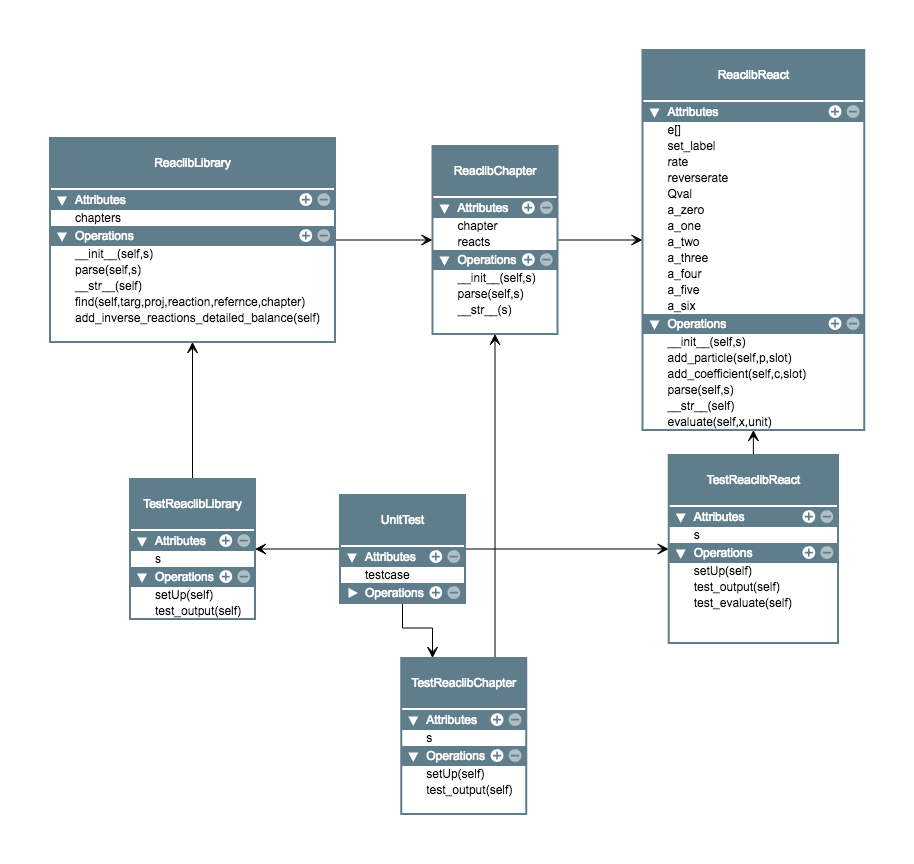
\includegraphics[width=\linewidth]{UML.png}
 \caption{This is a Unified Modeling Language (UML) diagram for the Python code written to output REACLIB 2 format. The headings in blue are the classes that format the REACLIB file. {\fontfamily{qcr}\selectfont ReaclibLibrary} splits the library into individual reactions and inputs this into the other two classes {\fontfamily{qcr}\selectfont ReaclibChapter} and {\fontfamily{qcr}\selectfont ReaclibReact} to be further evaluated. {\fontfamily{qcr}\selectfont ReaclibChapter} delegates which lines of reactions are chapter headings and which lines are the actual numbers contributing to the calculation of the ARR.  It will evaluate the different chapter headings and then output the reaction block to be passed onto the {\fontfamily{qcr}\selectfont ReaclibReact} class. This class will store each element of the reaction section as the number and position of projectiles, targets or ejectiles represents by {\fontfamily{qcr}\selectfont e[]}, a set label for citations, which type of rate the reaction is, the Q value of the reaction, and the seven parametrization constants. Unit tests are used to test each class of this code. The functions {\fontfamily{qcr}\selectfont gnds\_crossSection\_to\_Reaclib\_ARRcoefficients} and {\fontfamily{qcr}\selectfont gnds\_reactionSuite\_to\_ReaclibLibrary}, retrieve the cross section data from ENDF/B-VIII.0, after converting the data to the GNDS format using FUDGE GNDS file conversion. The  {\fontfamily{qcr}\selectfont numpy.linalg.lstsqr} function is used within the {\fontfamily{qcr}\selectfont gnds\_crossSection\_to\_Reaclib\_ARR\_coefficients} function to implement Eq. 5 from the cross section data. These individual functions do not belong to a class and are not explicitly shown on the UML diagram}
 \label{Figure 1}
\end{figure}
\begin{figure}
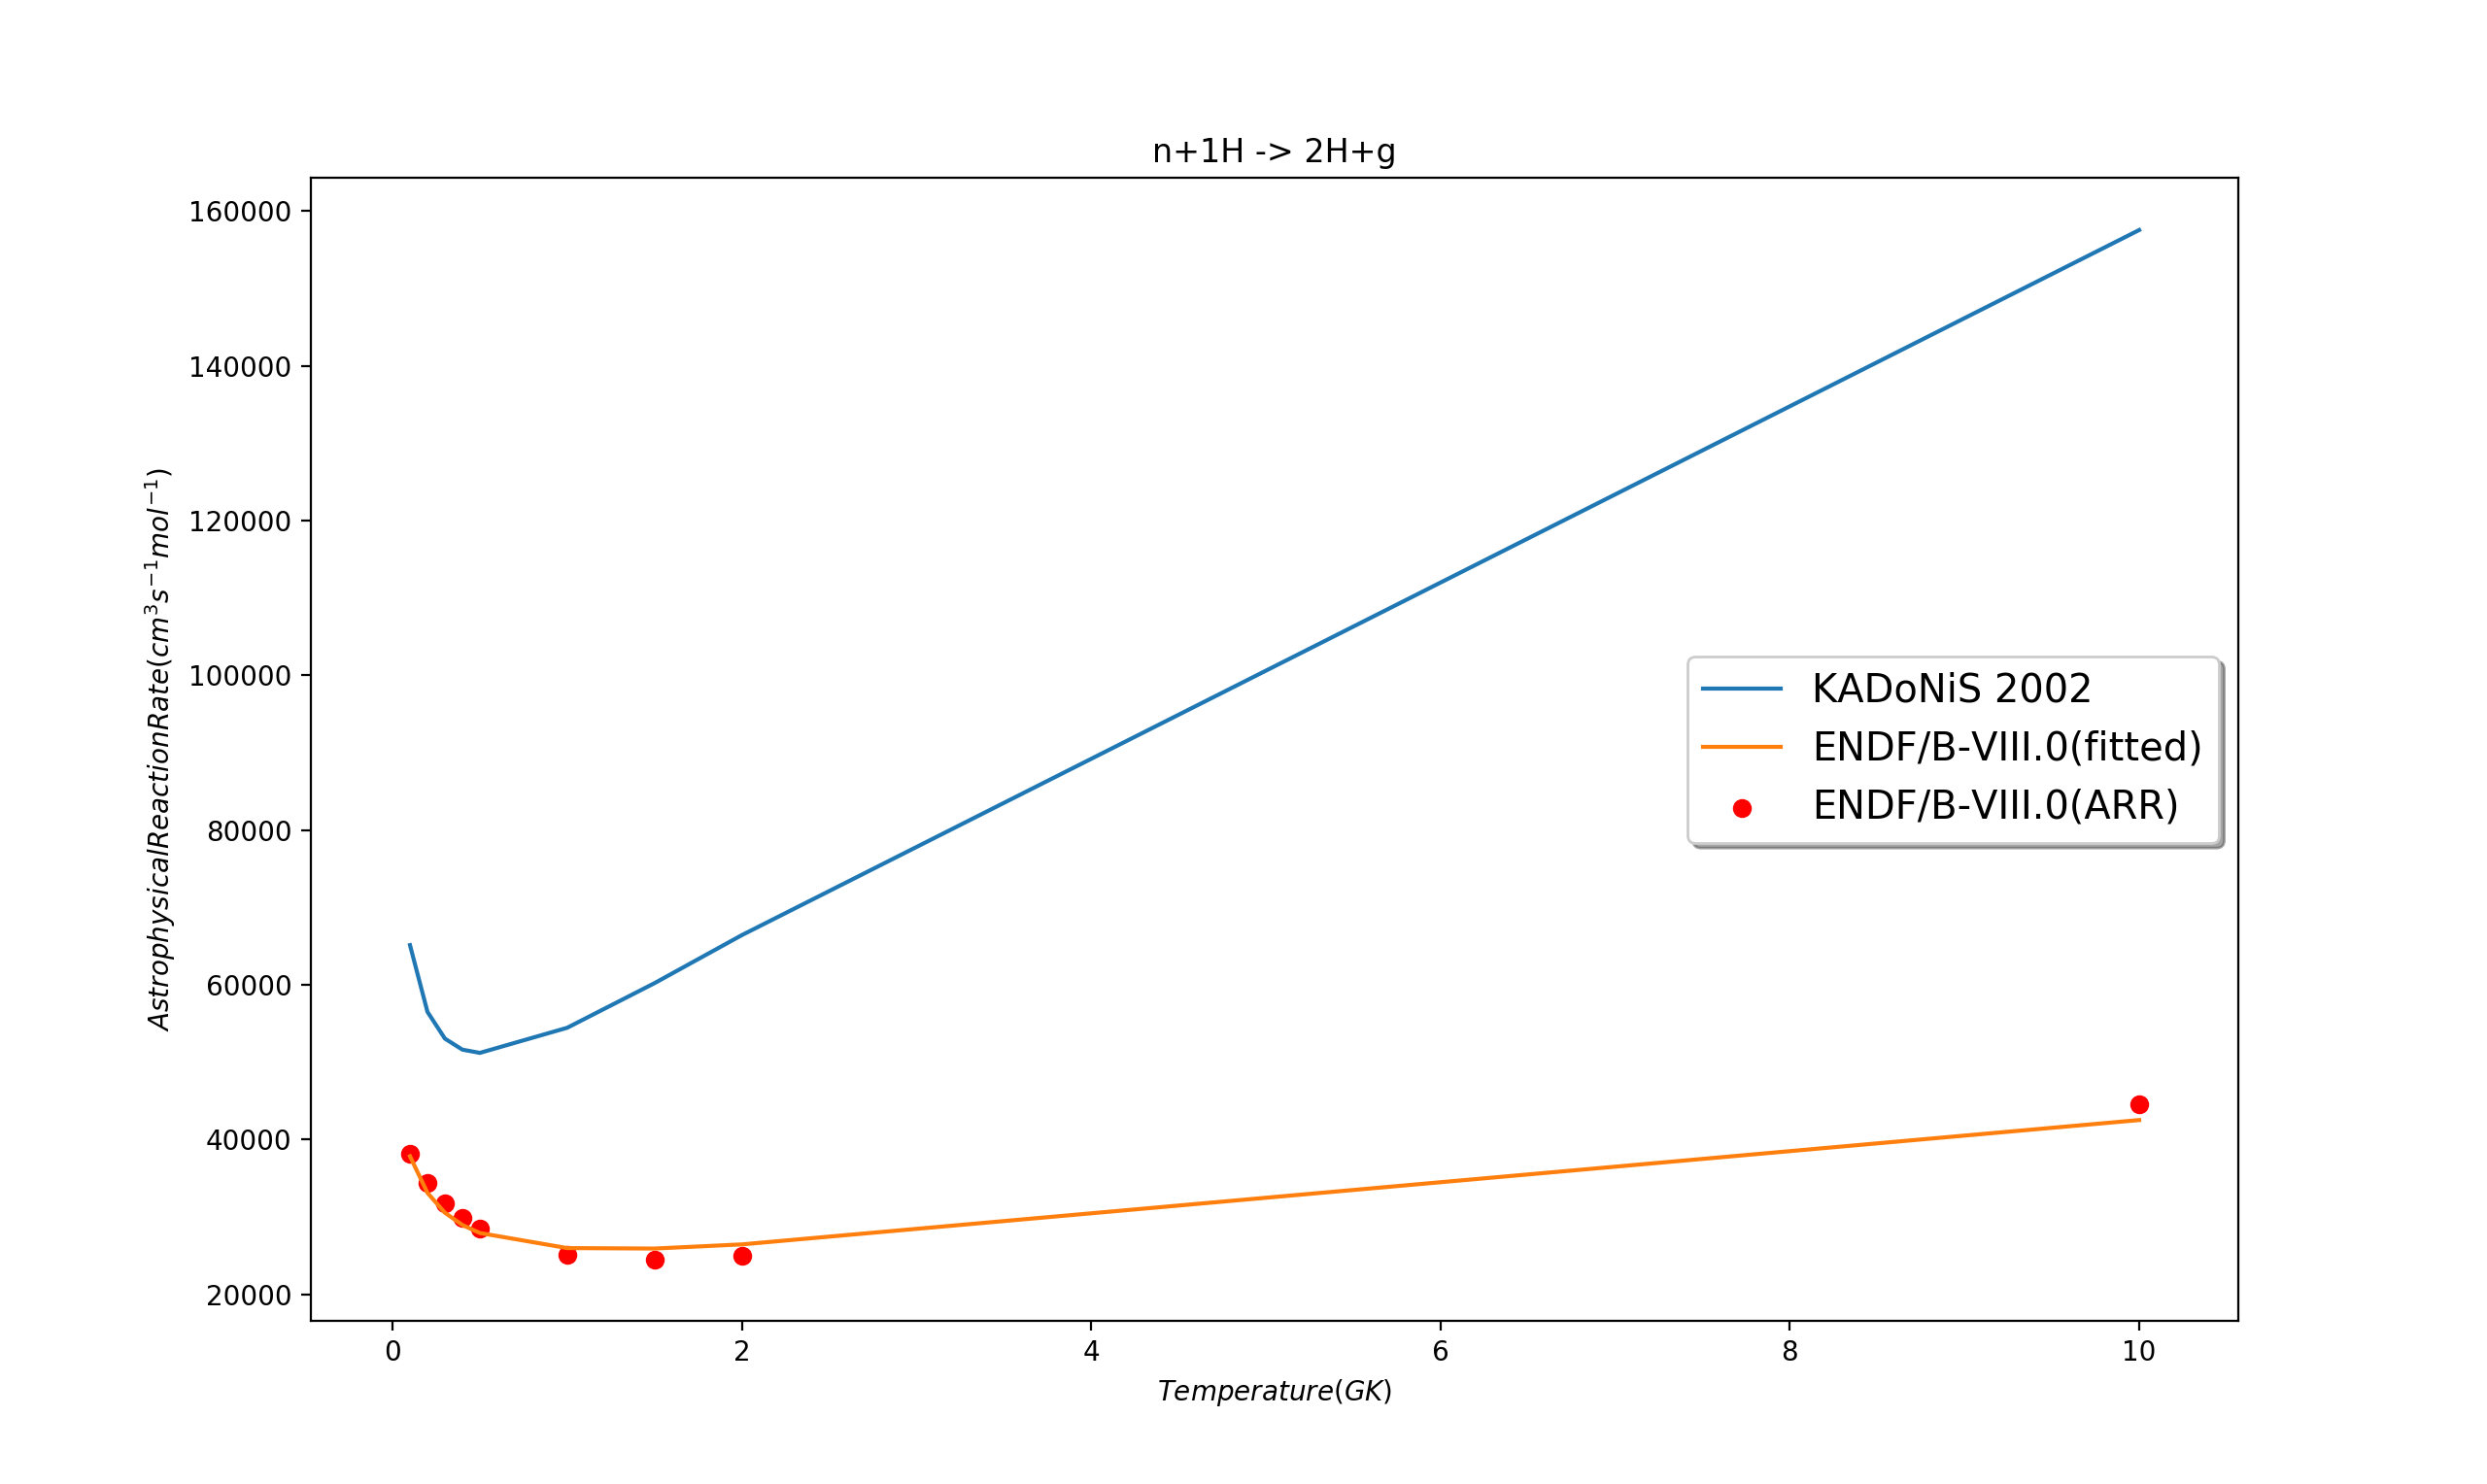
\includegraphics[width=\linewidth]{Hpng.png}
\caption{This figure shows the proton neutron capture reaction. This is an important reaction because it is the dominant mechanism for the production of Deuterium that occurs in the universe. This specific neutron capture reaction was a part of Big Bang nucleosynthesis, the foundation for all other nuclear reactions to occur. The figure shows that the KADoNiS rates, from SkyNet REACLIB, and ENDF/B-VIII.0 reaction rates are similar curves near the lower temperature range and diverge as temperature increases. The ENDF/B-VIII.0 reaction computed using the FUDGE ARR calculation has a strong overlap with the fitted ENDF/B-VIII.0 data from the REACLIB parametrization.
}
\end{figure}
\begin{figure}
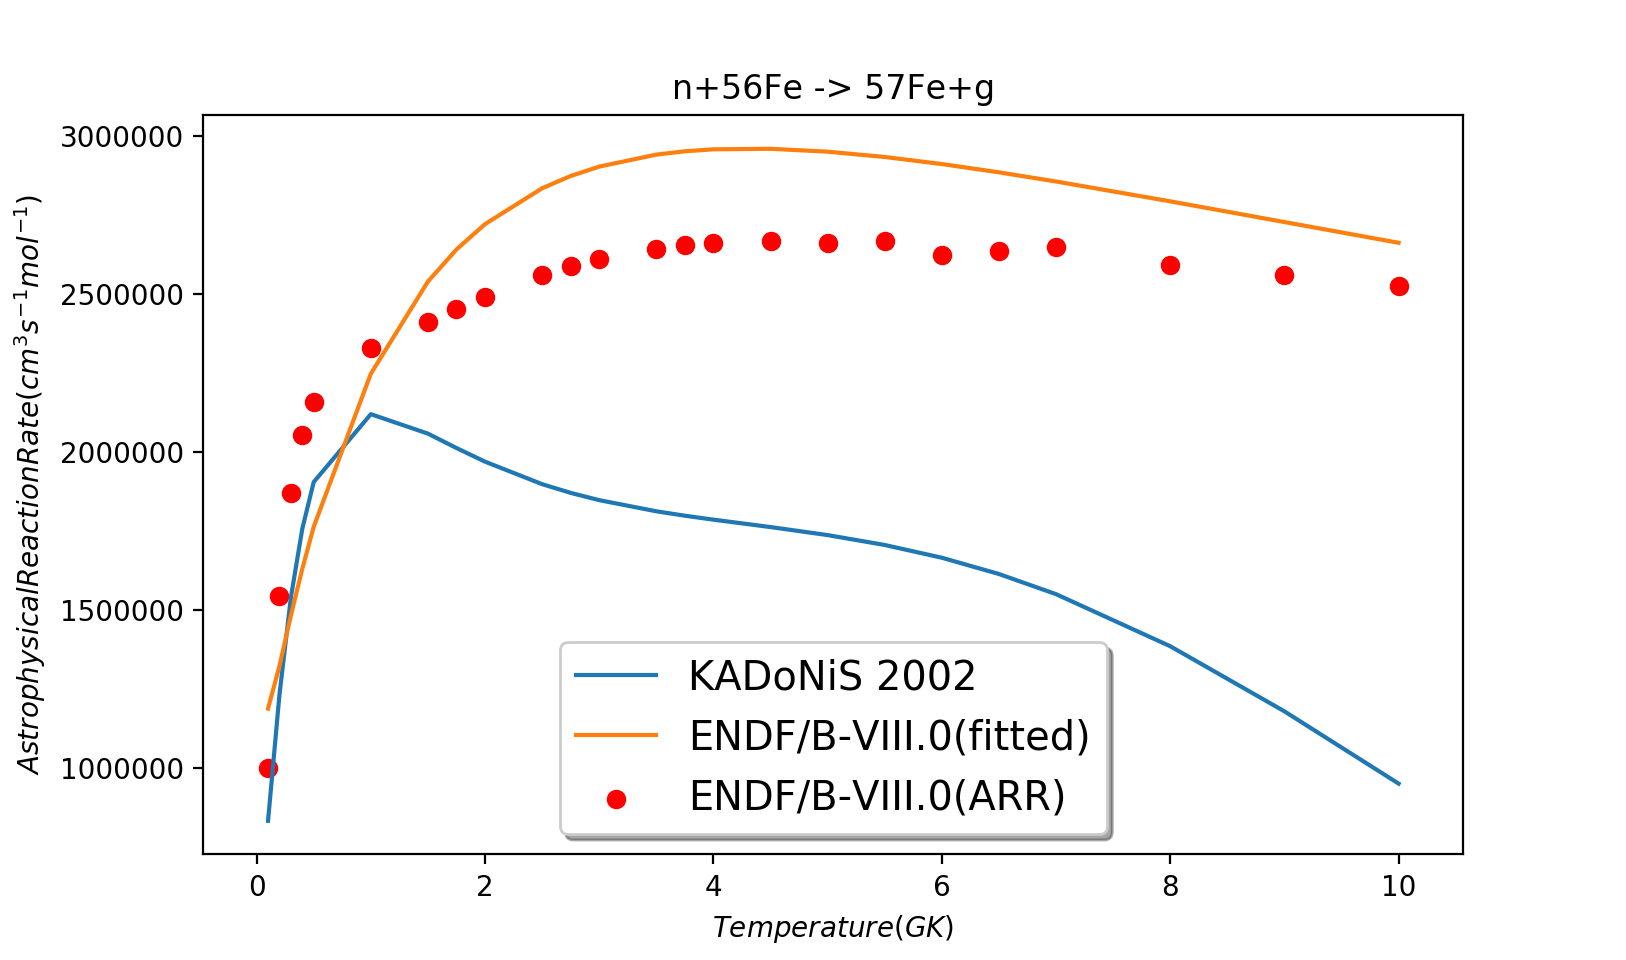
\includegraphics[width=\linewidth]{Fe56final.png}
  \caption{This figure shows the neutron capture reaction of $\prescript{56}{}{Fe}$. This reaction is vital to understanding stellar nucleosynthesis because Iron is the first of the heavy nuclei. This is noteworthy because the heavy nuclei are hypothesized to require the r-process from supernovae nucleosynthesis for formation formed rather than stellar nucleosynthesis which forms the lighter nuclei. This graph requires particular attention because it raises questions to the suitability of the fitting parameterization. The fitted ENDF/B-VIII.0 ARR and the FUDGE ARR from GNDS file of ENDF/B-VIII.0 have different curves. It is clear that there is a difference between the KADoNiS and ENDF/B-VIII.0 libraries that diverges as the temperature gets larger, but this trend is consistent with other reactions in the libraries, Fig. 2 and 4. But this graph is distinctive because the fitted ARR does not seem to be accurate. Further investigation into this discrepancy is needed. The general shape of the graph of FUDGE ARR and fitted ARR of ENDF/B-VIII.0 are similar but their comparative scale is not nearly as close as in figure 2 and 4.} 
  \label{Figure 3}
\end{figure}
\begin{figure}
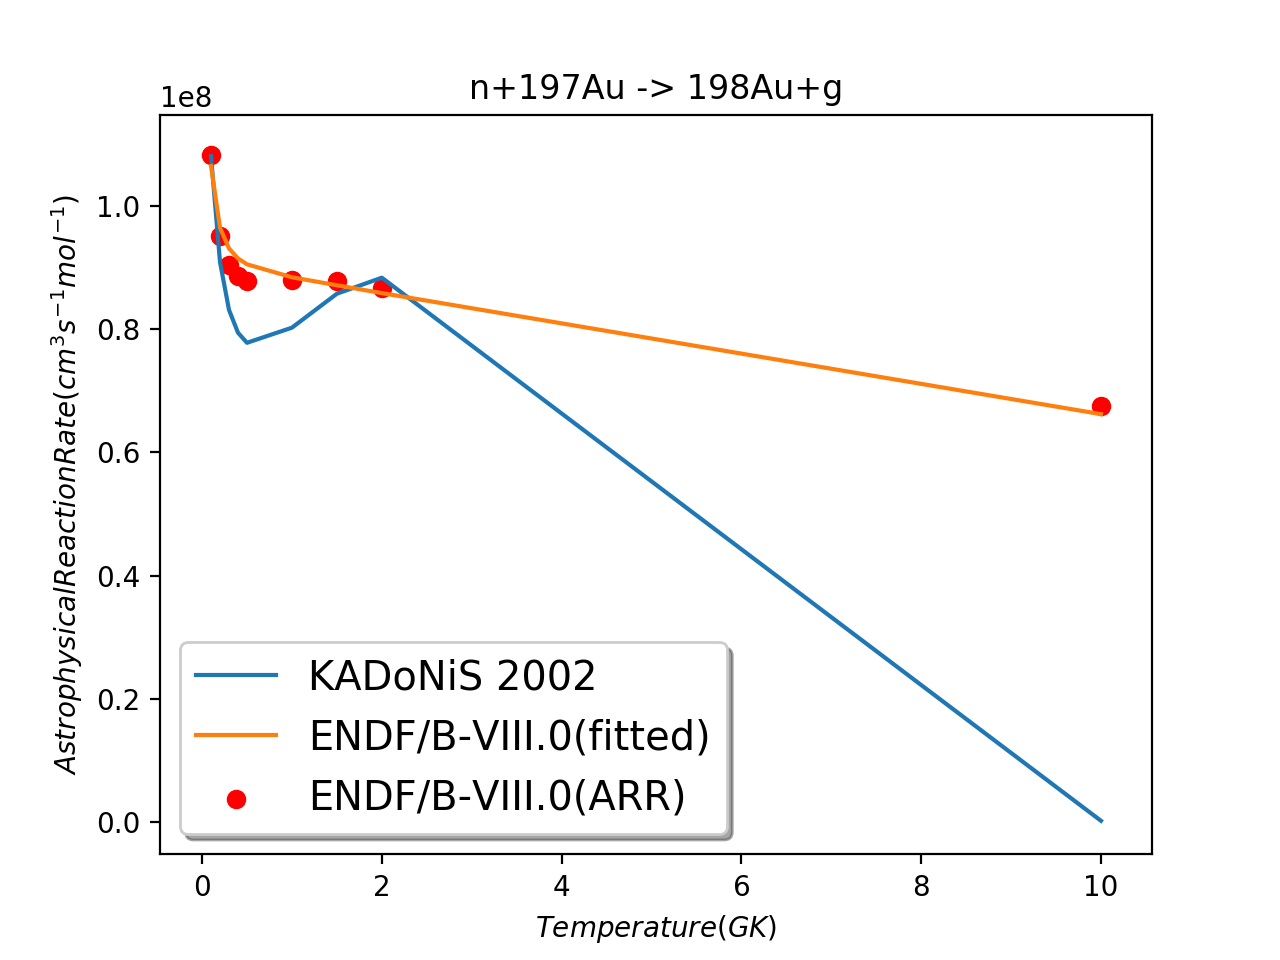
\includegraphics[width=\linewidth]{Au.png}
  \caption{This figure shows the neutron capture reaction for $\prescript{197}{}{Au}$. This is an important reaction because it is a neutron standard reaction that was recently re-evaluated. Yet, some astrophysical data libraries still use in-correct values, for example, KADoNiS. This figure exemplifies these incorrect values from KADoNiS. KADoNiS has an unclear peak in its data that does not match with ENDF/B-VIII.0, either fitted or unfitted.\cite{kadonis} This difference in the two libraries still diverges as the temperature increases as observed in Figure 2 and 3. The fitted ARR relatively matches the FUDGE computation of the ENDF/B-VIII.0 ARR, as it does in Figure 2. This graph supports the accuracy of the fitting procedure. } \label{figure 4}
\end{figure}
\begin{figure}
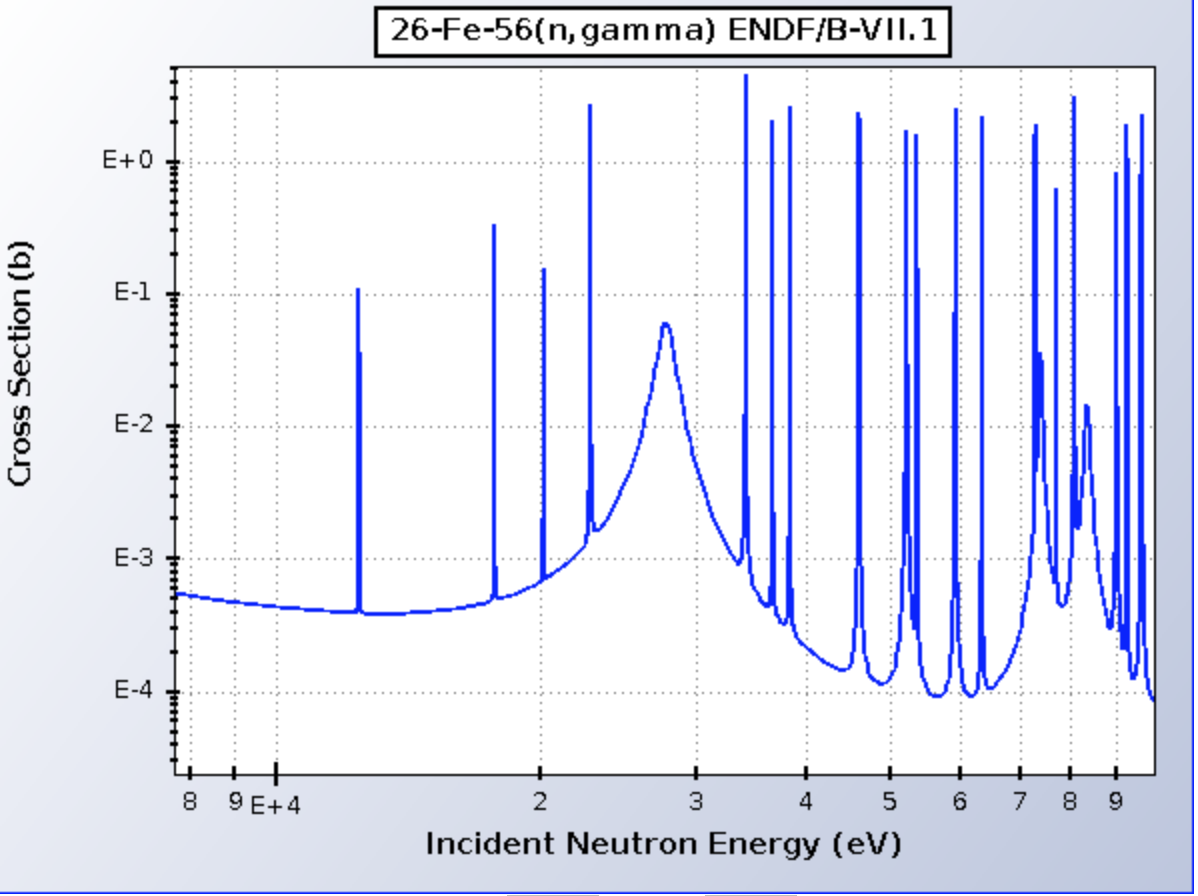
\includegraphics[width=\linewidth]{cross.png}
  \caption{This figure shows the neutron capture reaction for $\prescript{56}{}{Fe}$ from the National Nuclear Data Center at Brookhaven National Laboratory. This figure is zoomed in on the energy range relevant for the calculation of the ARR's needed for REACLIB format. The vertical axis plots cross sections and the horizontal axis plots energy in eV in the range of $0.1GK<T<10GK$. The gaps in the cross section at 30 keV make Iron very useful in experimentation, as it can be used to filter the energy of incident neutrons. This dip may have lead to the odd behavior of Figure 3.} \label{figure 4}
\end{figure}
\section{Acknowledgments}
I would like to give a special thanks to David Brown for welcoming me as a student intern and patiently guiding me through this entire project and invaluable summer experience. This project was supported in part by the U.S. Department of Energy under the Science Undergraduate Laboratory Internships Program (SULI).
\clearpage
%\printbibliography
\bibliography{biblio}
\end{document}

